\usepackage[utf8]{inputenc}
\usepackage[T1]{fontenc}
\usepackage[ngerman]{babel}
\usepackage{array}
\usepackage{bookmark}
\usepackage{textpos}
\usepackage{wasysym}
%\usepackage{listliketab}
\usepackage[NewCommands,NewParameters]{ragged2e}
\usepackage{tikz}
\usepackage{eurosym}
\usepackage{amssymb}
\usepackage{textpos}
%\usepackage{pstricks,auto-pst-pdf}
\usepackage{comment}

\usetheme{junghans}

\def\insertauthorindicator{Wer?}% Default is "Who?"
\def\insertinstituteindicator{Von?}% Default is "From?"
\def\insertdateindicator{Wann?}% Default is "When?"
\def\theDate{\today}

%\setbeamertemplate{caption}[numbered]

%%neuer Spaltentyp: linksb"undig + Silbentrennung
\newcolumntype{M}[1]{>{\RaggedRight\hspace{0pt}\arraybackslash}p{#1}}

\author{Marius Spix}

\institute[\raisebox{-4mm}{\includegraphics[width=1.9cm]{images/JW_Kontur}}]{
\includegraphics[scale=0.3]{images/J_60_Schwarz_Reflex_Blue}}
\title{QM-Cockpit}

%\addtobeamertemplate{frametitle}{}{
%\begin{textblock*}{100mm}(-4.15cm,-.55cm)
%\includegraphics[scale=.33]{images/Fahne2}\end{textblock*}
%}

\AtBeginSection{\frame{\sectionpage}}
%\AtBeginSubsection{\frame{\subsectionpage}}
\newtranslation[to=ngerman]{Section}{Abschnitt}
\newtranslation[to=ngerman]{Subsection}{Unterabschnitt}

\keywords{Abschlusspr\"{u}fung, Fachinformatiker, SAP, Quali\"{a}tsmanagement,
Lager, Warenwirtschaft}
\date{\theDate}

\frenchspacing

\begin{document}

\setcounter{framenumber}{0} 
\begin{frame}
  \maketitle
\end{frame}

\setcounter{figure}{0}

\begin{frame}{"Ubersicht}
  \tableofcontents
\end{frame}

\section{Projektumfeld}

\subsection{Betrieb}
\begin{frame}{Junghans Unternehmensgruppe}
	\begin{columns}
		\begin{column}{.45\textwidth}
			\includegraphics[width=\textwidth]{images/KarteJUG}
		\end{column}
		\begin{column}{.55\textwidth}
			\begin{block}{Fakten}
				\begin{itemize}
						\item Versandhandelsgruppe
						\item ca. 540 Mitarbeiter
				\end{itemize}
			\end{block}
			\vspace*{2ex}
			\begin{block}{}
				\hspace*{.37\textwidth}
				
\includegraphics[width=.63\textwidth]{images/J_60_Schwarz_Reflex_Blue}
				\\
				\includegraphics[width=.63\textwidth]{images/ProIdeeLogo}
			\end{block}
		\end{column}
	\end{columns}
\end{frame}

\subsection{Prozess}
\begin{frame}{Wareneingang}
 \begin{overlayarea}{\textwidth}{.42\textheight}
 	\only<1>{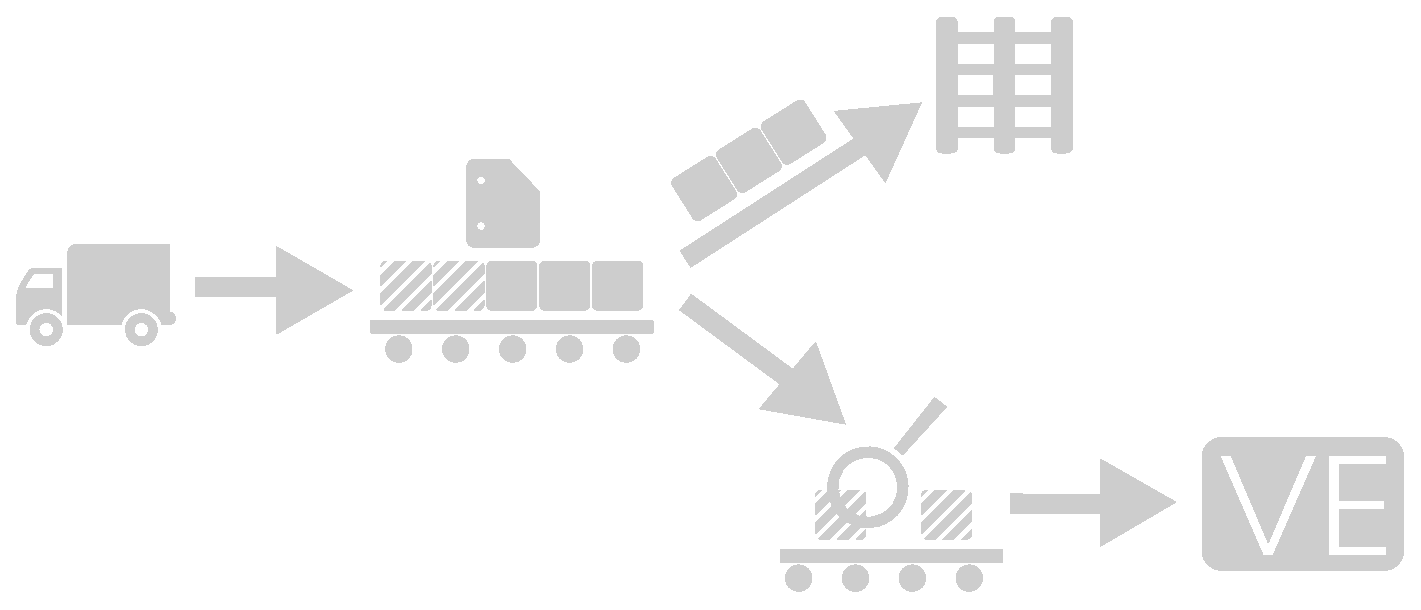
\includegraphics[width=.9\textwidth]{images/WE0a}<handout:0>}
 	\only<2>{\includegraphics[width=.9\textwidth]{images/WE1a}<handout:0>}
 	\only<3>{\includegraphics[width=.9\textwidth]{images/WE2a}<handout:0>}
 	\only<4->{\includegraphics[width=.9\textwidth]{images/WE3a}}
 \end{overlayarea}
 \begin{overlayarea}{\textwidth}{.58\textheight}
 \only<5->{
 	\vspace{-1ex}
 	\hrulefill
	\begin{columns}
		\begin{column}{.3\textwidth}
			\begin{minipage}[b]{\textwidth}
				\vspace{6\baselineskip}
				\centering
				\uncover<6->{\LARGE{600} \vspace{0pt} \normalsize{Anlieferungen}}
			\end{minipage}
		\end{column}
		\begin{column}{.4\textwidth}
 			\begin{figure}[tbh!]
 				\centering
				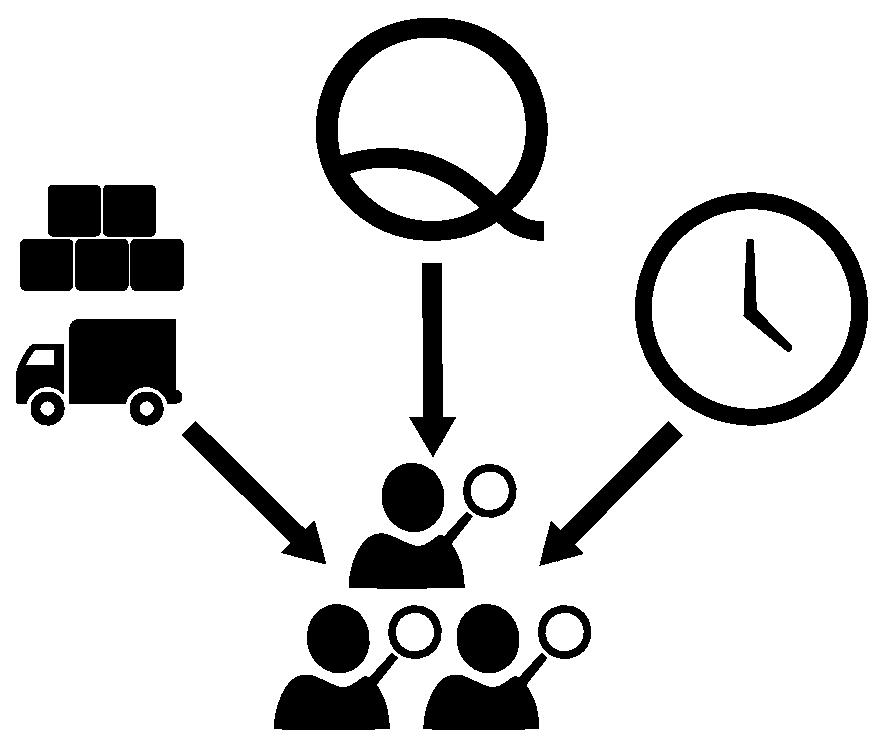
\includegraphics[width=\textwidth]{images/Kapazitaet}
 			\end{figure}
		\end{column}
		\begin{column}{.3\textwidth}
			\begin{minipage}[b]{\textwidth}
				\vspace{6\baselineskip}
				\centering
				\uncover<7->{\LARGE{2500} \vspace{0pt} \normalsize{Pr"uflose/Monat}}
			\end{minipage}
		\end{column}
	\end{columns}
 }
 \end{overlayarea}
\end{frame}

\section{Das Projekt}
\subsection{Ist-Analyse}
\begin{frame}[<+->]{Ist-Analyse}
	\begin{block}{Situation}
		\begin{itemize}[<+->]
			\item schwankender Personalbedarf
			\item {zeitaufw"andige, manuelle Personalplanung 
				\begin{itemize}
					\item Strichlisten, Excel-Tabellen \ldots
				\end{itemize}
			}
			\item {keine SAP-Standardfunktionalit"at}
			\item {zahlreiche Einflussfaktoren
				\begin{itemize}
					\item u.~A. "`Anwenderstatus"' der Pr"uflose \ldots
				\end{itemize}
			}
		\end{itemize}
	\end{block}
	\begin{block}{Auswirkungen}
		\begin{itemize}[<+->]
			\item unn"otiger organisatorischer Aufwand
			\item schlechte Kapazit"atsauslastung
			\item hohe R"uckst"ande
			\item Ursache nicht erkennbar
		\end{itemize}
	\end{block}

\end{frame}

\subsection{Soll-Konzept}
\begin{frame}[<+->]{Soll-Konzept}
	\begin{block}{Ziele}
		\begin{itemize}
			\item Zeitersparnis bei der Personalplanung
			\item Auswertung der abgeschlossenen Pr"uflose
			\item flexible Erweiterbarkeit
		\end{itemize}
	\end{block}
	\begin{block}{Abnahmekriterien}
		\begin{itemize}
			\item{spontane Auswertungen auf zeitnahen Daten
			\begin{itemize}
				\item nach Sortiment, VE, Anwenderstatus \ldots
			\end{itemize} }
			\item Ermittlung der Bearbeitungszeit
			\item{statistische Funktionen
			\begin{itemize}
				\item Z"ahlung der Pr"uflose
				\item summieren, filtern, gruppieren
				\item Erstellung von Diagrammen
			\end{itemize} }
		\end{itemize}
	\end{block}
\end{frame}

%\begin{comment}

\subsection{Durchf"uhrung}

\begin{comment}
\begin{frame}{Entwicklungsprozess}
 \vspace{2ex}
 \begin{overlayarea}{\textwidth}{\textheight}
  \only<1>{\includegraphics[width=\textwidth]{images/FDD1}<handout:0>}
  \only<2>{\includegraphics[width=\textwidth]{images/FDD2}<handout:0>}
  \only<3>{\includegraphics[width=\textwidth]{images/FDD3}<handout:0>}
  \only<4>{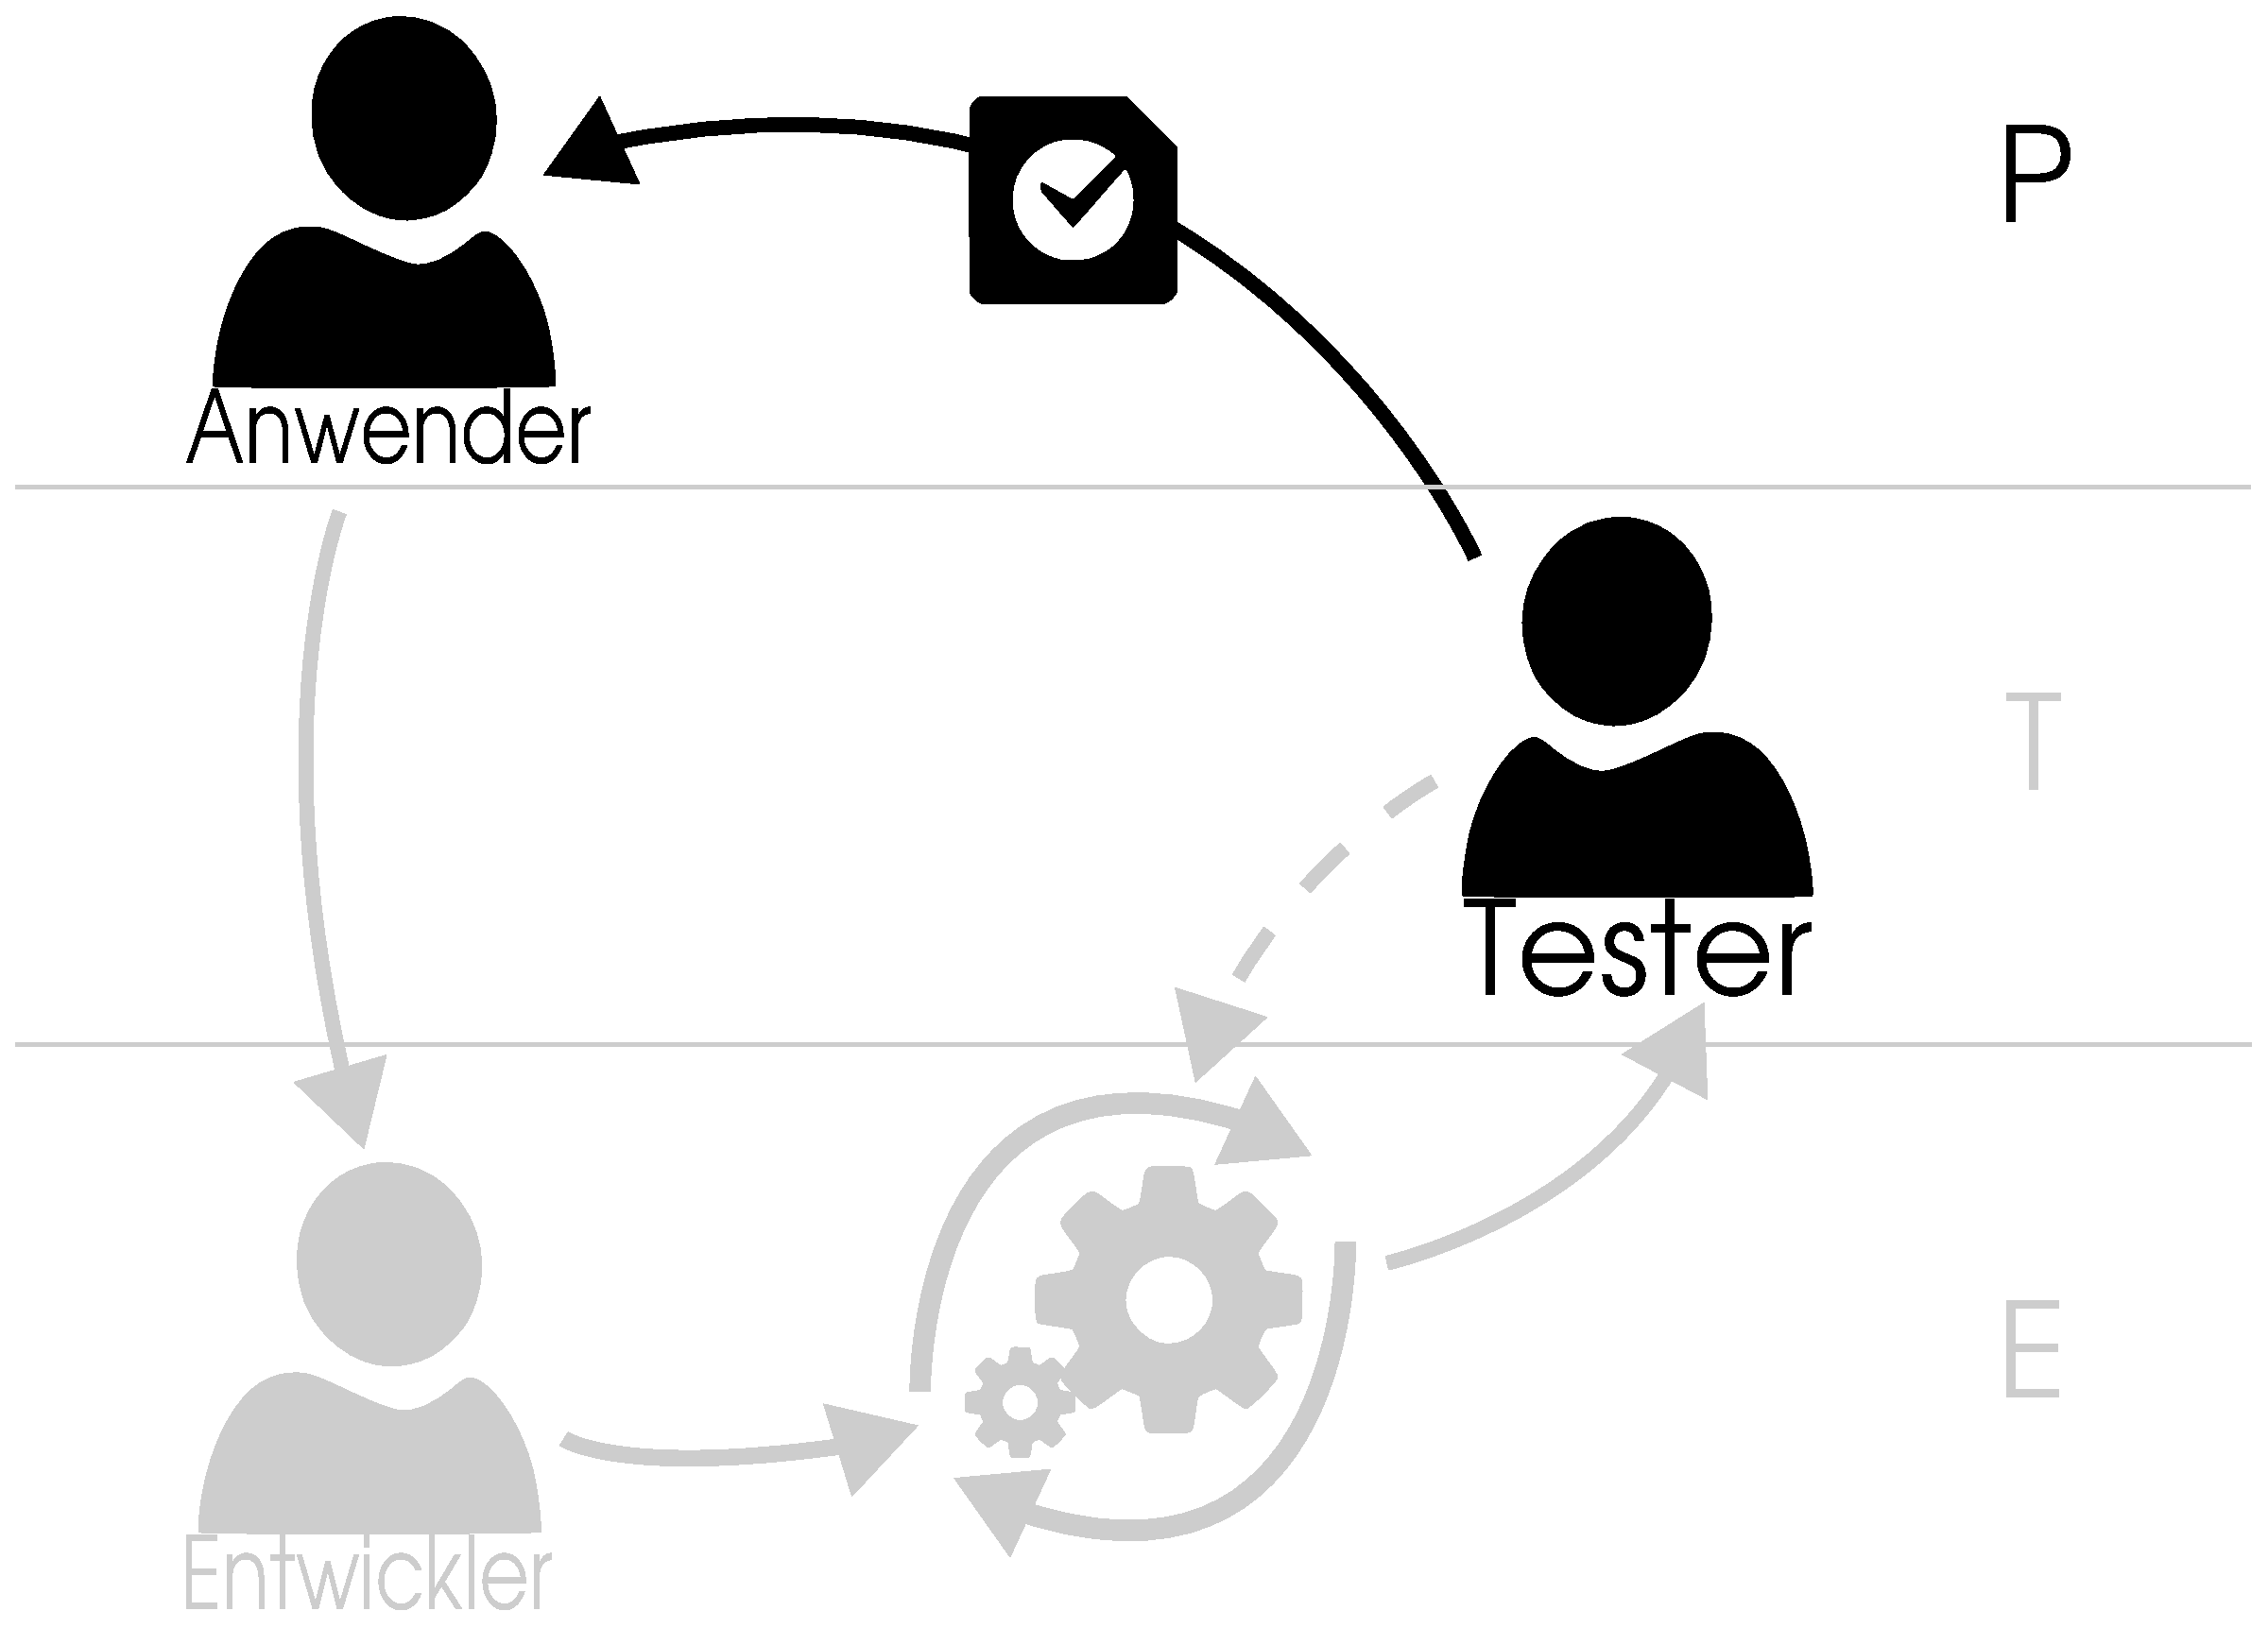
\includegraphics[width=\textwidth]{images/FDD4}<handout:0>}
  \only<5>{\includegraphics[width=\textwidth]{images/FDD5}}
 \end{overlayarea}
\end{frame}
\end{comment}

\begin{frame}{Modularer Aufbau}
\begin{figure}[tb]
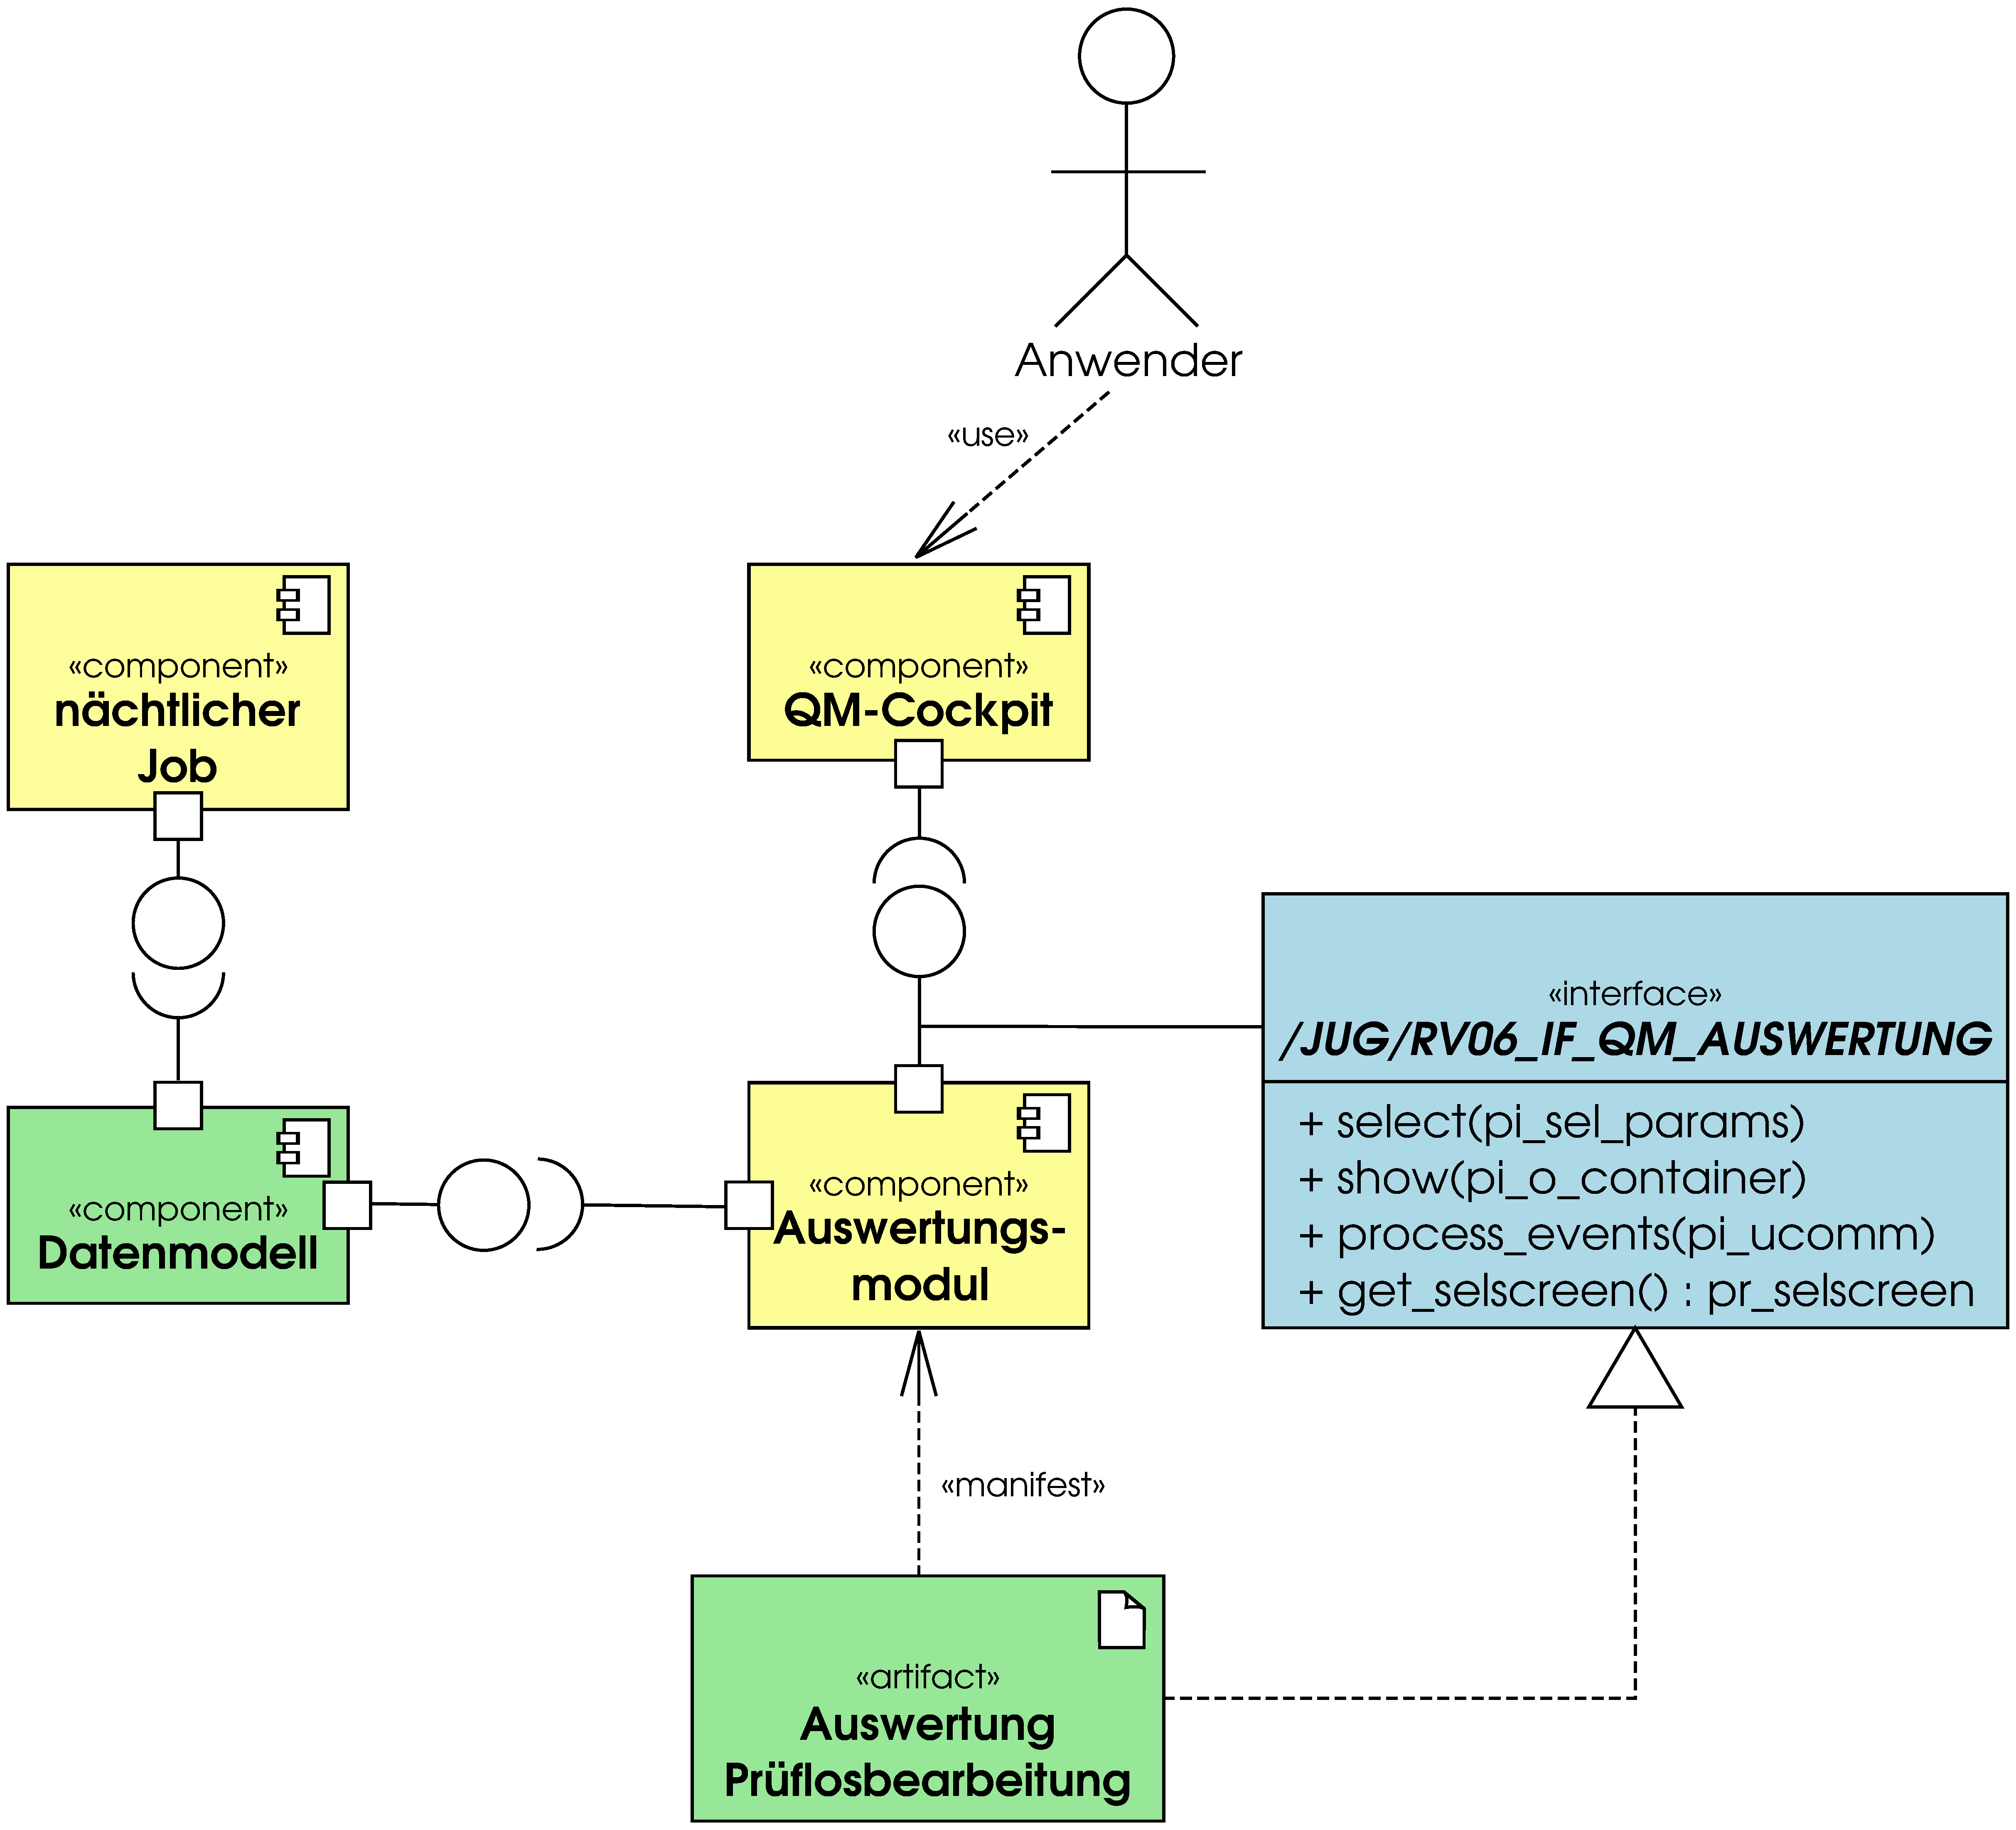
\includegraphics[width=.92\textwidth]{Komponenten}
\end{figure}
\end{frame}

\begin{frame}{Dynamische Erweiterbarkeit}
\begin{figure}[tb]
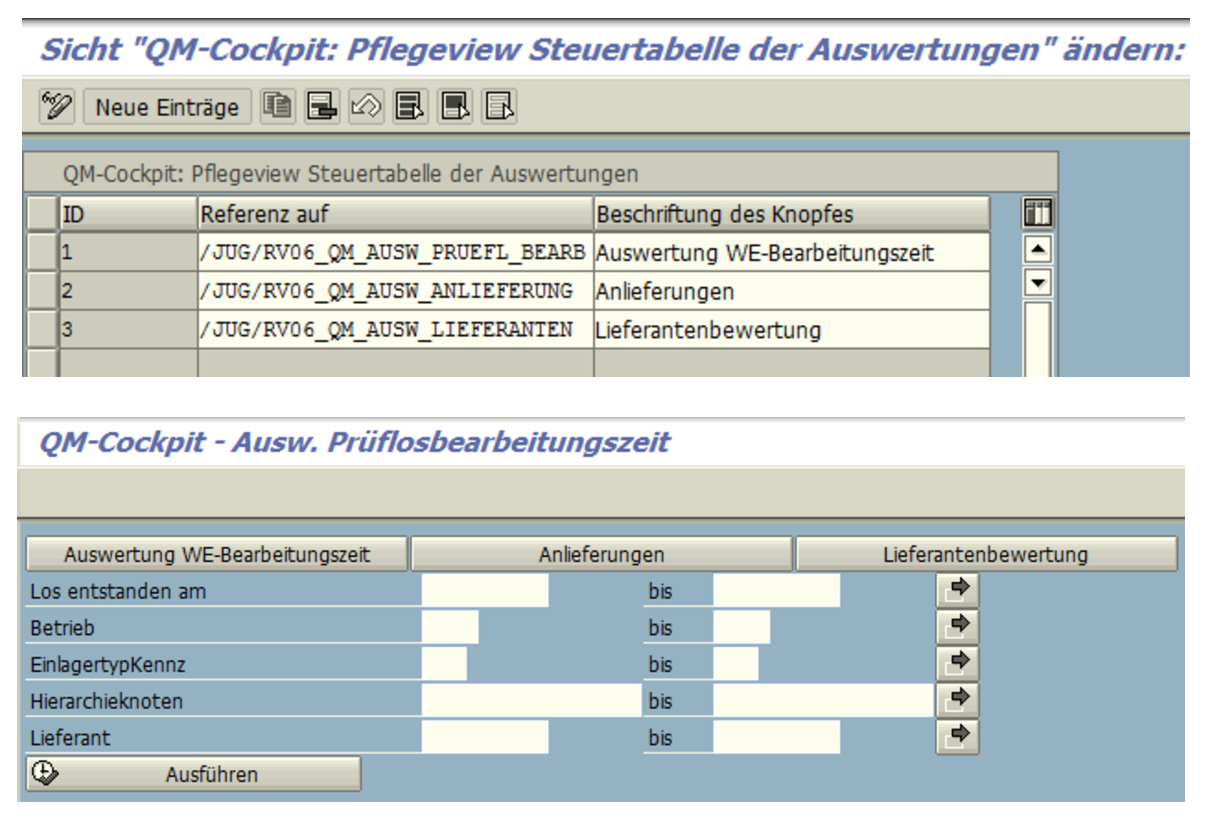
\includegraphics[width=\textwidth]{images/ErweiterbarkeitA}
\end{figure}
\end{frame}

\section{Ergebnis}
\subsection{Soll-Ist-Vergleich}
\begin{frame}{Ergebnis}
 \begin{overlayarea}{\textwidth}{.67\textheight}
   \vspace{3ex}
	\begin{figure}[b]
		\only<2>{\includegraphics[height=.48\textwidth]{images/Uhr}}

		\only<3-4> {
			\begin{columns}
				\begin{column}{.5\textwidth}
						
\includegraphics[width=.9\textwidth]{images/Strichliste}
				\end{column}
				\begin{column}{.5\textwidth}
					\alt<4>{
						\includegraphics[width=.9\textwidth]{images/QMCockpit2}}
						{\phantom{\includegraphics[width=.9\textwidth]{images/QMCockpit2}}}
				\end{column}
			\end{columns}
		}

		\only<5->{\includegraphics[height=.48\textwidth]{images/Kreisdiagramm}}
	\end{figure}
 \end{overlayarea}
 
 \begin{overlayarea}{\textwidth}{.33\textheight}
 \centering
 \only<2>{
	{\huge{69\,h Durchf"uhrungszeit}}
 }

\only<3-4> {
		\begin{columns}
			\begin{column}{.5\textwidth}
				{\huge{Vorher: $1 \frac{3}{4}$\,h}}
			\end{column}
			\begin{column}{.5\textwidth}
				 \only<4>{
					{\huge{Nachher: $\frac{1}{4}$\,h}}
 				}
			\end{column}
		\end{columns}
	}

 \only<5>{
	{\huge{86\,\% Zeitersparnis}}
 }
 \end{overlayarea}
\end{frame}

\begin{frame}{Einblicke}
	\begin{figure}[hbt!]
		\only<1>{\includegraphics[width=.92\textwidth]{images/QMCockpit2}}
		\only<2>{
			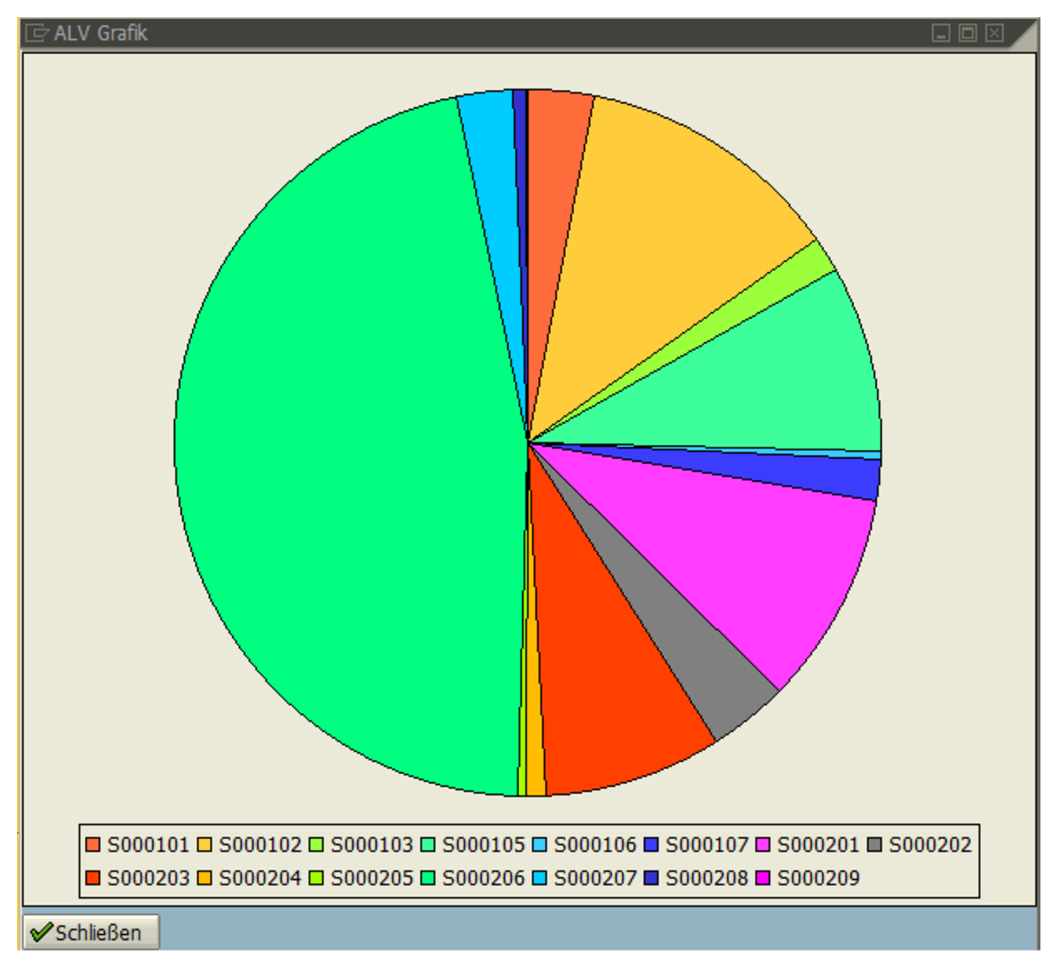
\includegraphics[width=.8\textwidth]{images/QMCockpit4}
		}
		\only<3>{
			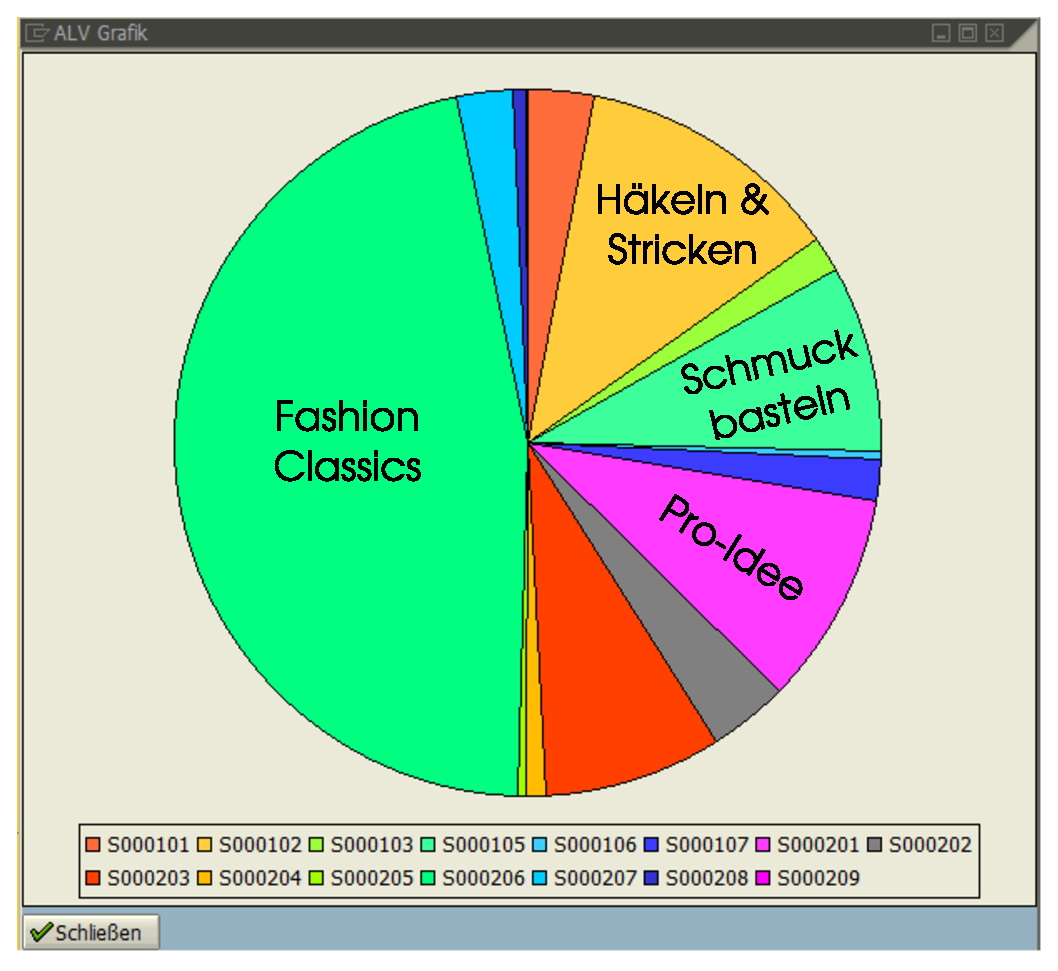
\includegraphics[width=.8\textwidth]{images/QMCockpit4a}
		}
	\end{figure}
\end{frame}

\subsection{Abschluss}
\begin{frame}[<+->]{Abschluss}
	\begin{block}{Soll-Ist-Vergleich}
		\begin{itemize}
			\item{Zeitersparnis bei der Personalplanung \checkmark}
			\item{Auswertung der abgeschlossenen Pr"uflose \checkmark}
			\item{flexible Erweiterbarkeit \checkmark}
		\end{itemize}
	\end{block}
	\begin{block}{Fazit}
		\begin{itemize}
			\item Integrationstest erfolgreich
			\item live seit 24.\,M"arz\,2014
			\item Fachbereich zufrieden
		\end{itemize}
	\end{block}
	\begin{block}{Ausblick}
		\begin{itemize}
			\item{weitere Auswertungen in Planung
				\begin{itemize}
					\item{geplante Anlieferungen}
					\item{Statistik zur Liefertreue}
				\end{itemize}
			}
		\end{itemize}
	\end{block}
\end{frame}

\begin{frame}{}
\begin{center}
\huge{Vielen Dank f"ur Ihre\\Aufmerksamkeit}\\
\begin{figure}[b!]

\includegraphics{images/platform11}
\end{figure}
\end{center}
\end{frame}

\end{document}

